\chapter{Mechanik eines einzelnen Massenpunktes}



\section{Schwere Masse und Tr"age Masse}

Grunds"atzlich muss man zwischen zwei verschiedenen Arten von Masse
unterscheiden:

\begin{description}[\setlabelstyle{\bfseries\slshape}]
\item[{Schwere Masse} $m_G$] Durch bspw. eine Balkenwaage vergleicht
   man die Masse des zu wiegenden St"ucks mit einer Referenzmasse --
   bspw. dem Urkilogramm (s. Def. \ref{def_kilogramm} auf
   S. \pageref{def_kilogramm}). Beide Massen befinden sich im gleichen
   Schwerefeld.

\item[{Tr"age Masse} $m_T$] Das Massenteil wird bspw. zwischen zwei
   Federn eingespannt und zu Schwingungen angeregt. Es gilt $T \sim
   \sqrt{m_T}$ mit der tr"agen Masse $m_T$ und der Periodendauer
   $T$. Nun vergleicht man die Periodendauer einer Masse in diesem
   Aufbau mit der Periodendauer bspw. des Urkilogramms.
\end{description}
Die beiden Messmethoden verwenden zum Vergleich verschiedene
Eigenschaften des K"orpers. Mathematisch nicht zu beweisen, jedoch
durch zahlreiche Experimente untermauert ist nun die Formel
$$
\boxed{m_T = m_G = m}
$$
Dieser Zusammenhang wird auch \textbf{"Aquivalenzprinzip} genannt.

Man kann sogar sagen, dass die
\index{Gravitationskonstante}Gravitationskonstante $\gamma$ (auch $G$
genannt) so gew"ahlt wurde, dass f"ur die Zahlenwerte $m_T = m_G$
gilt.




\section{Kraft}

Kraft ist ein Vektor! Sie wird gemessen, indem man bspw. die
Verformung eines K"orpers betrachtet, an den diese Kraft angreift. Zwei
Kr"afte sind gleich, wenn sie die gleiche Richtung haben und wenn
sie bei dem K"orper die gleiche Verformung erwirken (also gleichen
\emph{Betrag} haben).








\section{Das \textsc{Newton}'sche Grundgesetz}\index{Newton}
\label{kap_newton}


\begin{Wichtig}[Tr"agheitsgesetz (I. \textsc{Newton}'sches Axiom)]
   \index{Newton I} Ein K"orper verharrt in Ruhe oder in
   gleichf"ormiger Bewegung wenn keine Kraft an ihn angreift.
\end{Wichtig}

\begin{Wichtig}[II. \textsc{Newton}'sches Axiom]\index{Newton
     II}
   Wenn ein K"orper beschleunigt werden soll, muss eine Kraft auf ihn
   einwirken.
\end{Wichtig}

Aus Experimenten ergibt sich, dass $a \sim F$ und $a \sim
\frac{1}{m}$. Kombiniert man diese beiden Formeln, so ergibt sich
$$
a \sim \frac{F}{m} ~\Rightarrow ~ F \sim m \cdot a
$$
Nun w"ahlt man die Krafteinheiten so, dass die
Proportionalit"atskonstante der Formel $1$ wird und schon hat man die
Ber"uhmte Formel von \textsc{Newton}:
\begin{Wichtig}[\textsc{Newton}'sche Grundgleichung]
\index{Newton'sche
     Grungleichung}\index{Newton II!Gleichung}
     \begin{equation}
          \boxed{
              F = m \cdot a
          }
          \label{eqn_newton}
     \end{equation}
\end{Wichtig}
bzw. mit Vektoren:
$$
\vec F = m \cdot \vec a
$$
und au"serdem hat man die Einheit der Kraft definiert:
\begin{Def}[Newton $\mathbf N$]\index{Newton (Einheit)}
     $1N = 1\frac{Kg \cdot m}{s^2}$
     
     Ein Newton ist die Kraft, die auf einen K"orper mit der Masse $1
     Kg$ wirken muss, damit dieser die Beschleunigung von $1
     \frac{m}{s^2}$ erf"ahrt.
\end{Def}
Damit ist die Einheit $N$ offensichtlich im MKS-System
(s. Kap. \ref{kap_mks-system}).


K"orper auf der Erde erfahren abh"angig von ihrer Masse eine Kraft in
Richtung des Erdmittelpunktes. Diese Kraft wird \textbf{Schwerkraft}
genannt. Nach der oben gefundenen Formel \ref{eqn_newton} entspricht
diese Kraft einer Beschleunigung in Richtung des Erdmittelpunktes. Wir
bemerken diese, wenn ein K"orper f"allt.
\begin{Def}[Erdbeschleunigung $\mathbf g$]
   Ein K"orper in der N"ahe der Erdoberfl"ache wird mit der
   Beschleunigung $g$ in Richtung des Erdmittelpunktes
   beschleunigt. Dabei ist $g$ von der Masse der K"orper unabh"angig!
     
   Man kann rechnen $F_g = m \cdot g$ und hat mit $F_g$ die
   \textbf{Gewichtskraft}, die auf einen K"orper wirkt. \footnote{Diese
     \emph{Linearisierung} der Erdanziehungskraft ist eigentlich nur
     eine N"aherung: Entfernt man sich weiter vom Erdboden oder begibt
     sich darunter, wird die Formel immer ungenauer. Siehe dazu
     Kap. \ref{kap_schwerkraft}.}
\end{Def}



\begin{Wichtig}[actio = reactio (III. \textsc{Newton}'sches
   Axiom)]\index{Actio}\index{Reactio}\index{Newton III}
   "Ubt ein K"orper $A$ eine Kraft $F_A$ auf den K"orper $B$ aus, so "ubt
   gleichzeitig $B$ auf $A$ eine Kraft $F_B$ aus. Die beiden Kr"afte
   haben dabei den gleichen Betrag und entgegengesetzte Richtungen,
   greifen jedoch an \emph{verschiedenen} K"orpern an!\footnote{Es
     handelt sich also nicht um ein Kr"aftegleichgewicht!}
     \begin{equation}
          \boxed{actio = reactio}
         \label{eqn_actio-reactio}
     \end{equation}
\end{Wichtig}






\subsection{Verschiedene Arten von Kr"aften}
\label{kap_arten_von_kraeften}

Wir unterscheiden im Allgemeinen zwischen

\begin{description}[\setlabelstyle{\bfseries\slshape}]
\item[Gewichts-/Schwerkraft]  Siehe Kap. \ref{kap_schwerkraft}
\item[Reibunsgkr"afte] \index{Reibungskraft}
Sie wirken entgegengesetzt der Bewegungsrichtung $\Vec v$.

   Mikroskopische Ursache sind kleinste Unebenheiten in K"orpern, die
   sich verzahnen und bei Bewegung muss diese Verzahnung "uberwunden
   werden. Ruht der K"orper, muss man
   \textbf{Haftreibung}\index{Haftreibung} "uberwinden, gleitet er
   \textbf{Gleitreibung}\index{Gleitreibung} und rollt er
   \textbf{Rollreibung}\index{Rollreibung}.

   All diese Reibungen sind innerhalb bestimmter Grenzen von der
   Geschwindigkeit unabh"angig zur Normalkraft $F_N$, mit der sie
   \emph{senkrecht} auf die Oberfl"ache gedr"uckt werden, proportional:
\begin{equation}
   \label{eqn_reibung}
   F_R = \mu \cdot F_N
\end{equation}
dabei ist $\mu$ der entsprechende Reibungskoeffizient und eine
Materealkonstante und unabh"angig von der Auflagefl"ache der K"orpers.
\item[Zentripetalkraft] Sorgt daf"ur, dass ein K"orper auf seiner
   Kreisbahn bleibt.

   Siehe Kap. \ref{kap_kreisbewegung-i}
\item[Federkraft] Es gilt das 
   \begin{Def}[\textsc{Hook}'sche Gesetz]
\index{Hook'sches Gesetz}\label{def_hook-sches-gesetz}
      Die L"ange $x$, um die eine Feder verformt wird, ist proportional
      zur ben"otigten Kraft $F_D$:
      \begin{equation}
         \label{eqn_hooksches-gesetz}
         F_D = - D \cdot x
      \end{equation}
      mit der \textbf{Federkonstanten} $D$ ($[D] = \frac{N}{m}$)
   \end{Def}
\item[Scheinkr"afte] Siehe Kap. \ref{kap_scheinkraefte}
\end{description}










\section{Schwerkraft}
\index{Schwerkraft}\label{kap_schwerkraft}


\begin{Def}[Schwerkraft]\label{def_schwerkraft}\label{def_gravitation}
     Die Schwerkraft ist eine von vier fundamentalen Kr"aften in der Physik! 
     
     Zwischen zwei K"orpern mit Masse besteht eine Anziehung -- diese
     wird \textbf{Schwerkraft} genannt.
\end{Def}

F"allt ein K"orper (oBdA ein Apfel) auf die Erde, so tut er das, weil
er von der Erde eine Kraft -- eben $F_g$ -- erf"ahrt und so in
Richtung der Erde beschleunigt wird. Gleichzeitig erf"ahrt die Erde
aber auch eine Kraft in Richtung Apfel. Wegen $actio = reactio$ gilt
nun
$$
F_1 = F_2 ~ \Leftrightarrow ~ m_A \cdot a_A = m_E \cdot a_E
$$
Nun ist aber $m_E \gg m_A$ und damit $a_A \gg a_E$. D.h. die Erde
f"allt auch -- nur sehr wenig.




\subsection{Messung von Schwerkraft -- Gravitationswaage}

In Abb. \ref{img_schwerkraftwaage} ist eine Skizze einer
\textbf{Gravitationswaage}. Hier l"asst man die beiden gro"sen Massen
$M$ zuerst weg und schaltet den Laser ein. Wenn man die Massen $M$
dann zugibt, werden die kleinen Kugeln $m$ von ihnen angezogen und die
ganze aufgeh"angte Apparatur dreht sich -- eben auch der Spiegel. So
wird der Laserstrahl abgelenkt. "Uber den Winkel kann man das
Drehmoment der Bewegung bestimmen -- und dadurch die Anziehungskraft
zwischen $m$ und $M$.

\begin{figure}
     \centering
     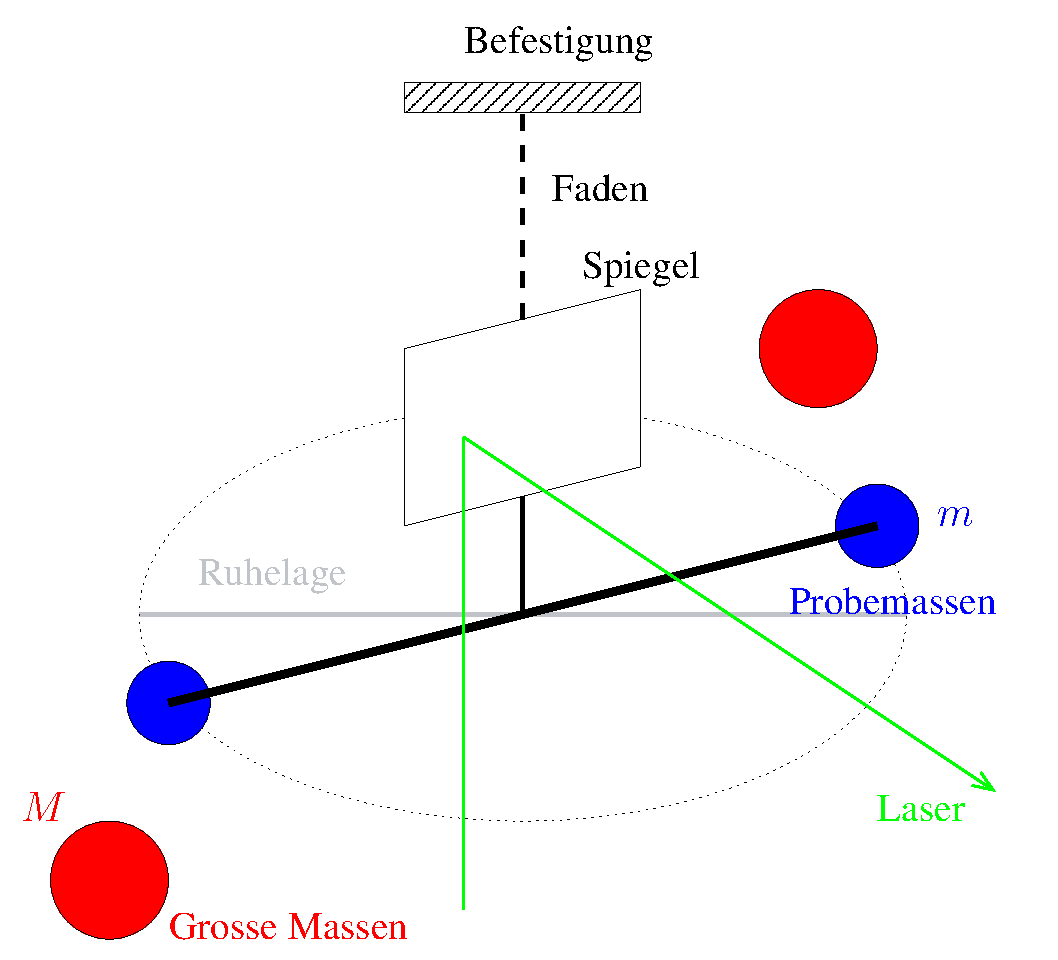
\includegraphics[width=0.7\textwidth]{bilder/gravitationswaage02}
     \caption[Gravitationswaage]{Die Massen $M$ lenken die Massen $m$
       ab, diese Drehen den Spiegel und ein Laserstrahl wird abgelenkt
% A: Aufh"angung, darunter der Faden. S: Spiegel; am Faden
%        befestigt. m: kleine Massen -- durch ein Gest"ange am Faden
%        befestigt. M: gro"se Massen, feste Positionen. 
}
     \label{img_schwerkraftwaage}
\end{figure}





\subsection{Berechnung der Schwerkraft}
\label{kap_scherkraft_berechnung}


Die Gravitationskraft zwischen zwei K"orpern kann man berechnen mit 
\begin{equation}
   \label{eqn_gravitation}
   \boxed{
      F = \gamma \cdot \frac{m_1 \cdot m_2}{r^2}
   }
\end{equation}
Dabei ist $r$ der Abstand zwischen den Massen $m_1$ und $m_2$ und $\gamma$ die
\begin{Def}[Gravitationskonstante $\gamma$ oder $G$]
\index{Gravitationkonstante}\label{def_gravitationskonstante}
   Die \textbf{Gravitationskonstante} ist eine Naturkonstante. Sie
   betr"agt
$$
 \gamma = 6,67 \cdot 10^{-11} \frac{m^3}{kg \cdot s^2}
$$
\end{Def}
Hieraus kann man auch einfach die Erdbeschleunigung berechnen:
$$
  F_G = m \cdot \underbrace{\frac{m_\text{Erde} \cdot \gamma}{r_E^2}}_g
$$
Hier kann man sehen, dass dies nur eine N"aherung ist, wenn
ein K"orper sich weiter von der Erdoberfl"ache entfernt.



\section{Scheinkr"afte}
\label{kap_scheinkraefte}

\begin{Def}[Inertialsystem]
\index{Inertialsystem}\label{def_inertialsystem}
Es treten nur dann Beschleunigungen auf, wenn Kr"afte wirken
\end{Def}

Man befindet sich dagegen in \emph{keinem} Inertialsystem, sondern in
einem \textbf{beschleunigten Bezugssytem}, wenn die
\emph{Newton}'schen Axiome scheinbar verletzt werden. 

Wird ein Wagen beschleunigt, so sind die K"orper darin tr"age und wollen
auf der Stelle verharren -- so sieht es ein Au"senstehender. Ein
Mitbewegter dagegen denkt, die K"orper w"urden sich bewegen -- also muss
auf sie eine Kraft wirken. Diese Kraft ist eine
\textbf{Scheinkraft}. Der Mitbewegte kann dabei nicht erkennen, woher
diese Kraft kommt. Der Mitbewegte befindet sich also \emph{nicht} in
einem Inertialsystem.


\abs
Wir untersuchen als Spezialfall ein \textbf{Rotierendes System:}

\begin{Wichtig}[Rotierender Vektor]
\index{rotierender Vektor}
   Rotiert ein Vektor $\Vec r = \vec r(t)$ mit $\Vec \omega = \vec \omega(t)$, so gilt
   \begin{equation}
      \label{eq:425}
      \boxed{
\frac{\diff \Vec r}{\diff t} = \vec v = \Vec \omega \times \Vec r
}
   \end{equation}
Mit der \textbf{Rechten-Hand-Regel} gilt also: $\Vec \omega$: Daumen,
$\Vec r$: Zeigefinger, $\frac{\diff \Vec r}{\diff t}$: Mittelfinger.
\end{Wichtig}

% Hat man also ein um $\Vec \omega$ rotierendes System $S'$ und ein
% ruhendes System $S$, in denen sich ein Vektor $\Vec r$ bewegt, so
% beschreibt man diese Bewegung in $S'$ durch
% $$
%  \frac{\diff \Vec r^*}{\diff t} = \Vec v - \Vec \omega \times \Vec r 
% = \frac{\diff \Vec r}{\diff t} - \Vec \omega \times \Vec r \textcolor{red}{\text{ist das dann nicht =0?}}
% ~
%  \text{ bzw. } ~ 
%  \frac{\diff \Vec v^*}{\diff t} = \Vec a - \Vec \omega \times \Vec v = 
% \frac{\diff v}{\diff t} - \Vec \omega \times \Vec v
% $$
% wobei $\Vec v$ im System $S$ beschrieben ist und durch $\Vec \omega
% \times \Vec r$ noch die Rotation von $S'$ ausgeglichen
% wird\footnote{Bewegt sich bspw. ein K"orper mit der Rotation von $S'$,
%   so sind die Zahlen, die seine Position in $S'$ beschreiben
%   \emph{kleiner} als die in $S$ -- deshalb muss man hier die Rotation
%   abziehen.} -- als Ergebnis hat man die Bewegung in $S'$
% beschrieben.

% M"ochte man nun die Kr"afte auf ein Massenteilchen in $S$ und in $S'$
% beschreiben, so erh"alt man wegen $\Vec r' = \Vec r$ den Zusammenhang
% $$
%  \Vec  F' = m \cdot \Vec a + 2 m \cdot ( \Vec \omega \times \vec V ) + m
%   \cdot \Vec \omega \times ( \Vec \omega \times \Vec r )
% $$
% \textcolor{red}{\text{warum ist hier $\Vec r' = \Vec r$, was ist $\Vec V ?$}}
% Es wirkt ja eigentlich nur die Kraft $\Vec F = m \cdot \Vec
% a$. D.h. der restliche Term muss den Scheinkr"aften zugeordnet
% werden. Man nennt sie 

Wir wollen nun einen Vektor $\vec R$ betrachten; er kann ruhen oder
sich bewegen. Diesen Vektor $\vec R$ stellen wir nun mithilfe zweier
Koordinatensystemen $S$ und $S'$ dar, wobei $S'$ konstant mit $\vec
\omega$ rotiert und $S$ in Ruhe ist.

Wir nennen die Basisvektoren in $S$ $e_i$ und die Basisvektoren in
$S'$ hei"sen $\varepsilon_i$ (auf Vektorpfeile wollen wir hier
ausnamsweise der "Ubersichtlichkeit halber verzichten); die
Koeffizienten in $S$ entsprechend $x^i$ und die in $S'$ hei"sen
$\xi^i$. Damit k"onenn wir den Vektor $\vec R$ in den beiden Systemen
schreiben als
\begin{equation*}
   \vec R = \sum_i x^i e_i \text{ und } \vec R = \sum_i \xi^i\varepsilon_i
\end{equation*}
Nun wollen wir die Ableitung von $\vec R$ betrachten und wenden dabei
die \emph{Produktregel} zum Ableiten an.

In $S$ beachtet man dabei, dass die $e_i$ ruhen, also dass $\dot e_i = 0$.
\begin{equation*}
   \frac{\diff }{\diff t}\vec R = \sum_i \dot x^i e_i + x^i \dot e_i =
   \sum_i \dot x^i e_i
\end{equation*}
In $S'$ gilt dies dagegen nicht. Daf"ur k"onnen wir mit
Gl. \eqref{eq:425} $\dot \varepsilon_i = \omega \times \varepsilon_i$
schreiben:
\begin{equation*}
   \frac{\diff }{\diff t} \vec R = \sum_i \dot \xi^i \varepsilon_i +
   \xi^i \dot \varepsilon_i = 
\sum_i \dot \xi^i \varepsilon_i +
   \xi^i \omega \times \varepsilon_i =
\sum_i \dot \xi^i \varepsilon_i +
    \omega \times (\xi^i \varepsilon_i )
\end{equation*}
F"ur die zweite Ableitung gilt entsprechend:
\begin{equation*}
   \frac{\diff ^2}{\diff t^2} \vec R = \sum_i \ddot x^i e_i
\end{equation*}
und im System $S'$ (hier verwenden wir, dass $\frac{\diff }{\diff t}
\omega = 0$ ist):
\begin{equation*}
     \frac{\diff ^2}{\diff t^2} \vec R =
\sum_i \ddot \xi^i\varepsilon_i + 2 \cdot \dot \xi^i \dot \varepsilon_i +
\xi^i\ddot \varepsilon_i =
\sum_i \ddot \xi^i\varepsilon_i + 2 \cdot \omega \times (\dot \xi^i  \varepsilon_i) +
\omega \times (\omega \times (\xi^i \varepsilon_i ))
\end{equation*}

Verwenden wir nun noch die Schreibweise $\vec x = \sum_i x^ie_i$ und
$\vec \xi = \sum_i \xi^i \varepsilon_i$ erhalten wir f"ur die
Beschleunigung von $\vec R$:
\begin{equation}
   \label{eq:426}
   \frac{\diff ^2}{\diff t^2} \vec R = \ddot{ \vec x} = \ddot{\vec
     \xi} + 2 \cdot \vec \omega \times \dot{\vec \xi} + \vec \omega \times (
   \vec \omega \times \vec \xi)
\end{equation}
D.h. die \emph{Kraft}, die im System $S$ zu sp"uren ist, ist schlicht
$ m \cdot \ddot{\vec x}$. Im System $S'$ aber:
\begin{equation}
   \label{eq:427}
   \vec F' = m \cdot  \ddot{\vec \xi} = m \cdot \left (\ddot{\vec x} -   2 \cdot \vec \omega \times \dot{\vec \xi} - \vec \omega \times (
   \vec \omega \times \vec \xi) \right )
\end{equation}
D.h. im beschleunigten System nimmt man mehr Kr"afte wahr, als im
ruhenden System. Man unterscheidet:


\begin{description}
\item[Corioliskraft]
\index{Corioliskraft}
\begin{equation}
   \label{eqn_coriolis-kraft}
\boxed{   \Vec F_C = -2 m \cdot ( \Vec \omega \times \vec v ) }
\end{equation}
Sie tritt auf, wenn ein K"orper sich senkrecht zur Rotationsrichtung
eines (mit Drehfrequenz $\Vec \omega$) rotierenden Systems
bewegt, also wenn $\vec \omega \times \vec v \neq 0$ ist. Dazu muss
$\vec \omega$ nicht konstant sein!

Bewegt sich bspw. ein K"orper (von au"sen beobachtet) gerade auf einer
rotierenden Scheibe nach au"sen, legt er (f"ur den Mitrotierenden)
au"sen an der Scheibe eine weitere Strecke seitw"arts als in der
Scheibenmitte zur"uck. Er muss also durch eine (Schein-)kraft seitlich
beschleunigt worden sein; der Corioliskraft. 


\item[Zentrifugalkraft]\index{Zentrifugalkraft} oder
   \textbf{Fliehkraft}\index{Fliehkraft}
\begin{equation}
   \label{eqn_zentrifugalkraft}
 \boxed{   -m\Vec \omega \times ( \Vec \omega \times \Vec r ) }
\end{equation}
Sie tritt in jedem rotierenden System auf und ist die (Schein-)Kraft, die
der Mitrotierende daf"ur verantwortlich macht, dass die Dinge nach
au"sen gezogen werden, obwohl diese ja eigentlich nur tangential nach
au"sen wegfliegen wollen. Sie ist vom Betrag her gleich der
Zentri\emph{petal}kraft, also der Kraft, die einen K"orper auf einer
Kreisbahn h"alt (s. \ref{kap_kreisbewegung-i}). Man kann sagen, dass
die Zentrifugalkraft die Reaktio der Zentripetalkraft ist.
\end{description}










\section{Energieerhaltungss"atze}
\label{kap_energieerhaltungssaetze}


\begin{Def}[Arbeit]
   \index{Arbeit}\label{def_arbeit}
Es wird die \textbf{Arbeit} $W$ verrichtet, um einen K"orper gegen die
Kraft $\Vec F(\Vec r)$ auf der Bahn $\Vec r(t)$ (mit der L"ange $s$ zwischen
Startpunkt $a$ und Endpunkt $e$) zu
bewegen:
\begin{equation}
   \label{eqn_def_arbeit}
   W  = \int_a^e \Vec F(\Vec r) \, \diff \Vec r
\end{equation}
\end{Def}
Die Einheit der Arbeit ist $[W] = J = N \cdot m = W \cdot s$

Eine Anschauliche Folgerung hieraus: \textbf{Das goldene Gesetz der
  Mechanik}
\begin{quote}
   Man braucht die gleiche Energie, um einen K"orper die Strecke $s$
   mit der Kraft $F$ zu bewegen, wie wenn man den K"orper doppelt so
   weit mit der halben Kraft bewegt
\end{quote}
(um $n \cdot s$ mit der Kraft $\frac{1}{n} \cdot F$ bewegt).



\begin{Def}[Konservative Kraft]
\index{Konservative Kraft}\label{def_konservative-kraft}
   Die zu verrichtende Arbeit h"angt nur vom Anfang und Ende der
   Bewegung ab -- nicht vom \emph{Weg}. 

   Rein Mathematisch kann man sagen, dass in diesem konservativen Kraftfeld die
   \textbf{Rotation verschwindet}: $\vec \nabla \times \Vec F(\Vec r) = 0$,
   bzw. dass jedes geschlossene Integral verschwindet (wenn man eine
   geschlossene Bahn f"ahrt, braucht man dazu insgesamt keine Arbeit):
   $\oint_\gamma \Vec F(\Vec r) \, \diff \Vec r = 0$
\end{Def}

Wird nun Arbeit entgegen einer konservativen Kraft verrichtet, so ist
die Arbeit in Form von \textbf{Potentieller Energie}\index{Potentielle
Energie} gespeichert. Man spricht dann auch davon, dass ein Teilchen,
welches man mit der Arbeit $W$ im konservativen Kraftfeld $F$ bewegt
hat, das \textbf{Potential} 
\begin{equation}
   \label{eqn_potential}
     E_{pot} = -W
\end{equation}
besitzt.
\emph{Beispiele} f"ur solche konservativen Kr"afte sind
\begin{itemize}
\item Schwerkraft
\item Elastische Federkraft
\end{itemize}
und \emph{Gegenbeispiele} sind
\begin{itemize}
\item Reibungskraft (Wegabh"angig)
\item \textsc{Lorentz}kraft (Geschwindigkeitsabh"angig)
\end{itemize}
Hier kann man auch sehen, dass bei einer nicht konservativen Kraft
die Arbeit sp"ater nicht mehr zur Verf"ugung steht.

\begin{Def}[Potenzielle Energie]
   \index{Potentielle Energie}\label{def_potentielle_energie} 
   Um die Potentielle Energie eines Teilchens in einem Kraftfeld
   allgemein zu bestimmen, ben"otigt man einen festen Bezugspunkt
   $P_0$. Nun gilt f"ur das Potential an einem Ort $Q$:
\begin{equation}
   \label{eqn_potential_allgemein}
   \boxed{E_{pot} = - \int_{P_0}^Q \Vec F(\Vec r) \, \diff \Vec r}
\end{equation}   
\end{Def}

Ein Teilchen wird sich in der Natur stets so bewegen, dass es
potentielle Energie abgibt; es strebt ein (potentielles)
\emph{Energieminimum}\index{Energieminimum} an. Es wird sich so stets
dorthin bewegen, wo die "Anderung des Potentials am st"arksten negativ
ist(wo die Abnahme des Potentials maximal ist).
Dies interpretieren wir als \emph{Kraft}.

Mathematisch kann man das auch so ausdr"ucken:
\begin{equation}
   \label{eqn_gradientenfeld}
   \Vec F = - \Grad E_{pot} = - \nabla E_{pot}
\end{equation}

Und auch die Umkehr gilt: Kann man ein Kraftfeld als Gradientenfeld
ausdr"ucken (kann man also Gl. \eqref{eqn_gradientenfeld} f"ur dieses
Kraftfeld aufstellen), so handelt es sich um eine konservative Kraft.



\begin{Wichtig}["Aquipotentialfl"achen]
\index{"Aquipotentialfl"achen}\label{def_aequipotentialflaechen}
In einem konservativen Kraftfeld findet man Stellen, an denen die
Potentielle Energie gleich ist. Diese Stellen kann man mit Linien verbinden und sie
bilden so eine Fl"ache. Innerhalb dieser Fl"ache kann man K"orper ohne
Arbeitsaufwand bewegen.   
\end{Wichtig}

Im Schwerefeld der Erde bspw. sind die "Aquipotentialf"achen
Kugelschalen mit dem Erdmittelpunkt im Zentrum. Anschaulich hei"st
dies, dass man keine Energie braucht, um die Schwerkraft zu
"uberwinden, wenn man sich auf einer Fl"ache bewegt, die einen
konstanten Abstand zum Erdmittelpunkt wahrt.



\begin{Wichtig}
   [\index{Konservative Kraft}Konservative Kraft] Folgende
   Eigenschaften sind "aquivalent:
   \begin{enumerate}
   \item Es existiert ein skalarfeld $V$ sodass $\vec F = -\vec\nabla V$
   \item Die Arbeit h"angt nur von Anfangs- und ENdpunkt ab: $W =
      \int_\gamma F\diff\vec s = -\left(V(\gamma^\text{Anfang}) -
         V(\gamma^\text{Ende})\right)$
   \item Die Rotation verschwindet: $\vec\nabla\times \vec F = \vec 0$
   \end{enumerate}
\end{Wichtig}











\abs
Neben der \emph{statischen} -- also nur ortsabh"angigen -- Potentiellen
Energie gibt es noch die 
\begin{Def}[Kinetische Energie]
   \label{def_kinetische-energie}\index{Kinetische Energie}
Damit bezeichnet man die Arbeit, die ben"otigt wird, um einen K"orper
mit Masse $m$ auf eine Geschwindigkeit $v$ zu beschleunigen. Dabei
gilt
\begin{equation}
   \label{eqn_def_kinetische-energie}
   \boxed{
       \frac{1}{2} \cdot m \cdot v^2 = E_{kin}
   }
\end{equation}
\end{Def}
Dies kann man aus \eqref{eqn_def_arbeit} herleiten. Verwendet man $F =
m \dot v$, braucht man dies nur noch mit $v$ zu multiplizieren und
erh"alt
\begin{equation*}
   F \cdot v = m \cdot \dot v \cdot v
\end{equation*}
und weil $v = \frac{\diff s}{\diff t}$ ist, k"onnen wir die Gleichung
mit $\diff t$ "`multiplizieren"' und das Integral "uber die Zeit
ziehen; es ergibt sich
\begin{equation*}
   \int F \frac{\diff s}{\diff t} \diff t = \int F \diff s = 
\int m \dot v v \diff t
\end{equation*}
Im letzten Integral haben wir das Produkt von "`Funktion"' $v$ und
"`innerer Ableitung"' $\dot v$ -- und damit geht die Aufleitung
einfach. Es ergibt sich \eqref{eqn_def_kinetische-energie}. Au"serdem
folgt f"ur eine konservative Kraft, dass man das Erste Integral als
Potentialdifferenz ausdr"ucken kann\footnote{Wir haben in der
  Herleitung unbestimmte Integrale verwendet -- jetzt setzen wir die
  Grenzen $r_1$ und $r_2$ bzw. $t_1$ und $t_2$ ein.}:
\begin{equation*}
   \Delta V  = \Delta E_\text{kin} \text{ oder } -(V_2 - V_1) = 
   E_\text{kin,2} - E_\text{kin,1}
\end{equation*}


Nun h"angen kinetische und potentielle Energie einfach zusammen:
\begin{Wichtig}[Energieerhaltung]
\label{def_energieerhaltung}\index{Energieerhaltungssatz der Mechanik}
\begin{equation}
   \label{eqn_energieerhaltung_mechanik}
   \boxed{
     E_{kin} + E_{pot} = const
}
\end{equation}
Sollte bei dem Vorgang Reibung auftreten, so muss man diese noch
einbeziehen; schlie"slich muss zur "Uberwindung der Reibung auch Arbeit
verrichtet werden:
$$
   E_{kin} + E_{pot} + E_{reib} = const
$$
\end{Wichtig}
















\section{Impulserhaltungssatz}
\label{kap_impulserhaltungssatz}

\begin{Def}[Impuls]
   \index{Impuls}\label{def_impuls}
Der Impuls $\Vec p$ ist definiert als
\begin{equation}
   \label{eqn_def_impuls}
   \Vec p = m \cdot \Vec v
\end{equation}
Um eine \textbf{Impuls"anderung} hervorzurufen ist eine Kraft n"otig
(siehe die \textsc{Newton}'schen Axiome ab S. \pageref{kap_newton}):
\begin{equation}
   \label{eqn_zshg_impuls-kraft}
   \Vec F = \frac{\diff \Vec p}{\diff t}
\end{equation}
\end{Def}
Mit der Einheit $[p] = \operatorname{N} \cdot \operatorname{s} =
\frac{\operatorname{kg} \cdot \operatorname{m}}{\operatorname{s}}$.

Anschaulich kann man sich den Impuls als \emph{Wucht} eines K"orpers
vorstellen.

Es gilt nun der
\begin{Wichtig}[Impulserhaltungssatz]
   \index{Impulserhaltungssatz}\label{def_impulserhaltungssatz}
Der Gesamtimpuls eines abgeschlossenen Systems ist f"ur alle Zeiten konstant!
\end{Wichtig}
Speziell hei"st das, dass die Summe der Impulse vor einem Ereignis
gleich der Summe der Impulse nach dem Ereignis ist.



\begin{Beispiel}
   \textbf{\index{Raketengleichung}Raketengleichung:} Wir betrachten
   eine Raktete der Masse $m = m(t)$, die sich mit der Geschwindigkeit
   $v = v(t)$ gegen ein Schwerefeld mit $F = m\, g$ bewegt. Um zu
   beschleunigen, st"o"st die Rakete nach hinten Gas mit der
   (bez"uglich der Rakete) konstanten Geschwindigkeit $w$.

   Wir betrachten die Situation aus der Sicht der Rakete -- diese Ruhe
   also. Auch wenn die Rakete beschleunigt, so werden wir doch zu jedem
   Zeitpunkt ein Inertialsystem finden, welches sich gleich mit der
   Rakete bewegt; damit k"onnen wir die \textsc{Newton}'schen Axiome
   verwenden.

   F"ur die Kr"afte auf die Rakete gilt also (die Impuls"anderung des
   Gases treibt die Raktet an, die Schwerkraft und die Tr"age Kraft
   bremsen sie):
   \begin{equation*}
    \frac{\diff }{\diff t} (m_G w)  -  \frac{\diff }{\diff t}(mv)  -
    mg = 0
   \end{equation*}
   Weil die Rakete ruht und weil je mehr Gas ausgesto"sen wird, die
   Rakete leichter wird ($m + m_G = \const$ und $\dot m = -\dot m_G$)
   folgt:
   \begin{equation*}
      -\dot m \, w   - m \,\dot v   - mg = 0
\text{ oder }
-w \frac{\dot m}{m} - g =  \dot v
   \end{equation*}
   Integration nach der Zeit (von $t_0$ bis $t$ ) liefert:
   \begin{equation}
      \label{eq:209}
     w\, \ln\frac{m_0}{m(t)} - g(t-t_0) + v_0 = v(t)
   \end{equation}
   Dabei nehmen wir N"aherungsweise an, dass die Kr"afte auf die
   Rakete nur von deren Masse abh"angen (nicht von der zur"uckgelegten
   Strecke).
\end{Beispiel}









\section{St"o"se}
\label{kap_stoesse}

Bei St"o"sen sind die Erhaltungss"atze aus den Kapiteln
\ref{kap_energieerhaltungssaetze} und \ref{kap_impulserhaltungssatz}
entscheidend.

Es gibt dabei zwei wichtige Arten von Sto"svorg"angen:
\begin{description}[\setlabelstyle{\bfseries\slshape}]
\item[inelastischer Sto"s] Hier wird ein Teil der Bewegungsenergie der
   Sto"spartner vor dem Sto"s umgewandelt in
   \begin{itemize}
   \item Reibungsw"arme
   \item Deformationsenergie
   \item Anregungszust"ande von Atomen
   \item etc.
   \end{itemize}
   Diese Gr"o"sen fasst man zu einer Energiemenge $Q$ zusammen.$$Q \neq
   0$$
\item[elastischer Sto"s] Hier wird die Bewegungsenergie der Sto"spartner
   vor dem Sto"s vollst"andig in Bewegungsenergie der Sto"spartner nach
   dem Sto"s umgewandelt.$$Q = 0$$
\end{description}

\abs
F"ur die Energiebilanz bei den Sto"svorg"angen gilt also allgemein (da $E
= \frac{1}{2} mv^2 = \frac{p^2}{2m}$):
$$
  \sum_i \frac{p_i^2}{2m_i} =   \sum_j \frac{\tilde p_j^2}{2m_j} + \mathbf Q
$$
wobei $p$ die Impulse \emph{vor} und $\tilde p$ die Impulse
\emph{nach} dem Sto"s sind.

D.h. wir d"urfen nur bei \emph{elastischen St"o"sen} den
Energieerhaltungssatz (Kap \ref{kap_energieerhaltungssaetze})
anwenden, weil wir wenn $Q = 0$ keine Energien unber"ucksichtigt
lassen, wenn wir lediglich potentielle und kinetische Energie der
Teilchen betrachten.












\begin{Wichtig}[Schwerpunkt]
\index{Schwerpunkt}\label{def_schwerpunkt}
   Der \textbf{Schwerpunkt} eines K"orpers ist mathematisch
   \begin{equation}
      \label{eqn_schwerpunkt}
      \Vec r_S = \frac{\sum_i m_i \cdot \Vec r_i}{\sum_i m_i}
   \end{equation}
(wobei man die Summen auch durch Integrale ersetzen kann)
   und anschaulich der Punkt, an dem man den K"orper auf einer
   Nadelspitze balancieren k"onnte -- auch wenn man dann mit der Nadel
   im Inneren des Stoffes herumfurwerken m"usste.
\end{Wichtig}
Entsprechend kann man auch \textbf{Schwerpunktgeschwindigkeit}
$$
  \Vec v_S = \frac{\diff \Vec r_S}{\diff t} = 
 \frac{\sum_i m_i \cdot \Vec v_i}{\sum_i m_i} =
\frac{\Vec P_S}{M}
$$
und analog \textbf{Schwerpunktbeschleunigung} bestimmen. In der
Mechanik reduziert man die Bewegung von K"orpern oft auf die Bewegung
ihrer Schwerpukte. Die Bewegung eines Schwerpunkts ist davon
unbeeinflusst, wie die einzelnen Teilchen des K"orpers Kr"afte
aufeinander auswirken. Um die Bewegung des Schwerpunkts zu "andern,
braucht man eine externe Kraft.

Als \textbf{Schwerpunktsystem} bezeichnet man ein System, bei der der
Schwerpunkt der betrachteten Teilchen stets den Ursprung bildet. Hier
verschwindet der Gesamtimpuls $\Vec P$ aller Massen des Systems: $\Vec
P = 0$. Deshalb sind solche Systeme f"ur die Untersuchtung von
Sto"sprozessen oft hilfreich.\footnote{Bspw wenn man untersuchen
  m"ochte, in welche Richtung eine Kugel eine ruhende anst"o"st, wenn sie
  nicht zentral auf diese prallt.}

\begin{Beispiel}
   Wir betrachten zwei Kugeln der Massen $m$ und $n$, die sich mit $v$
   bzw. $u$ bewegen 
%und so die Impulse $p =mv$ und $q = nu$ haben
   .  Diese sollen elastisch sto"sen. Wir begeben uns in das
   Schwerpunksystem, welches sich mit $V = \frac{mv + nu}{m+n}$
   bewegt, damit haben die Teilchen hier die Geschwindigkeit $v_s = v
   - V$ und $u_s = u - V$. Die Summe der Impulse vor und nach (mit $'$
   gekennzeichnet) dem Sto"s verschwindet, und die Energie ist
   erhalten. Damit ist
   \begin{equation*}
      mv_s' + nu_s' = 0 \text{ oder } v_s' = -\frac{n}{m}u_s' \text{
        und analog }      
 v_s = -\frac{n}{m}u_s
   \end{equation*}
In die Energierhaltung eingesetzt (Faktor $\frac{1}{2}$ gek"urzt)
\begin{equation*}
   mv_s^2 + nu_s^2 = m{v_s'}^2 + n{u_s}^2
\text{ folgt }
\frac{n^2}{m} {u_s}^2 + n{u_s}^2 = \frac{n^2}{m} {u_s'}^2 + n{u_s'}^2 
\text{ und so }
{u_s}^2 = {u_s'}^2
\end{equation*}
Das bedeutet $u_s' = \pm u_s$. Hier macht nur die "`$+$"'-L"osung
Sinn, weil die Kugel sonst einfach ungehindert weiterfl"oge. Analog
folgt $v_s' = - v_s$. Im Laborsystem ist also nach dem Sto"s: 
\begin{equation*}
   v' = v_s' + V \text{ und } u' = u_s' + V
\end{equation*}
\end{Beispiel}




\abs Um einen \textbf{Schwerpunkt} praktisch zu \textbf{bestimmen},
h"angt man den K"orper an verschiedenen Stellen auf und h"angt an die
Aufh"angung zudem ein Lot. Wiederholt man dies, schneiden sich die
beiden Lotlinien im Schwerpunkt.











\section{Drehimpuls}
\label{kap_drehimpuls}



Bisher hatten wir den Impuls als geradlinige Bewegungen betrachtet;
jetzt untersuchen wir ihn bei \emph{Rotationen}. In Analogie zum
Normalen Impuls (s. Def. \ref{def_impuls}) definiert man den
Drehimpuls $\Vec L$:

\begin{Def}[Drehimpuls]
   \index{Drehimpuls}\label{def_drehimpuls} Der
   \textbf{Drehimpuls} eines Teilchens mit Masse $m$ und
   Geschwindigkeit $\Vec v$ am Ort $\Vec r$
   \begin{equation}
      \label{eqn_def_drehimpuls}
      \Vec L = \Vec r \times (m \cdot \Vec v) 
       = \Vec r \times \Vec p 
        = m \cdot (\Vec r \times \Vec v)
   \end{equation}
\end{Def}

Der Drehimpuls ist von einer frei w"ahlbaren Achse bzw. dem
Koordinatenursprung abh"angig. Im Allgemeinen w"ahlt man die
Rotationsachse des K"orpers.  


$\Vec L$ steht senkrecht zu Bewegung $\Vec v$ und Ortsvektor $\Vec
r$. L"auft die Bewegung in einer Ebene ab, so k"onnen wir $\Vec v$
zerlegen -- $\vec v_\bot \bot \Vec r$ und $\vec v_\| \| \vec
r$. Wenden wir nun \eqref{eqn_def_drehimpuls} an, erhalten wir
\begin{equation}
   \label{eqn_differenz-c7}
   \Vec L = m ( \vec r \times (\vec v_\bot + \vec v_\|) = 
 m ( \vec r \times \vec v_\bot + \underbrace{\vec r \times \vec
   v_\|}_{\vec 0}) = m \cdot \vec r \times \vec v_\bot
\end{equation}
D.h. f"ur den Drehimpuls ist nur die Komponente \emph{senkrecht} zum
Ortsvektor entscheidend.

\begin{Wichtig}
   Bewegt sich ein Masseteilchen $m$ in einer Ebene, so zeigt $\Vec L$ stets in dieselbe \emph{Richtung} ($\frac{\Vec L}{\|\Vec L\|} = const$ aber
   $\|\Vec L\|$ muss nicht $const$ sein). 
\end{Wichtig}
Die Umkehr des Satzes gilt auch.



\begin{Def}
   [\index{Drehmoment}Drehmoment]\label{def_drehmoment}
   Das \textbf{Drehmoment} steht im gleichen Zusammenhang zum Drehimpuls, wie
   die Kraft beim gew"ohnlichen Impuls.
   \begin{equation}
      \label{eqn_def_drehmoment}
      \Vec M = \frac{\diff}{\diff t} \Vec L = \Vec r \times \Vec F
   \end{equation}
\end{Def}
Man kann dies analog zu $\frac{\diff p}{\diff t} = F$
\eqref{eqn_zshg_impuls-kraft} schreiben:
\begin{equation*}
   \label{eqn_differenz-c8}
   \frac{\diff \vec L}{\diff t } = 
m \cdot \left ( \underbrace{\frac{\diff \vec r}{\diff t} \times \vec
     v}_{\vec 0} + 
\vec r \times \frac{\diff \vec v}{\diff t} \right ) =
m \cdot ( \vec r \times \dot{ \vec v} ) = r \times (m\dot{\vec v}) = r
\times \dot{\vec p} = r \times \vec F
\end{equation*}
\begin{Wichtig}
   Um den Drehimpuls zu "andern, braucht man ein Drehmoment.
\end{Wichtig}


% Anschaulich kann man sich vorstellen, dass zu den wie beim
% gewohnlichen Impuls $\Vec p$ verarbeitetn Informationen "uber
% Geschwindigkeit und Masse durch die Information erg"anzt wird, wie weit
% die Masse von einem Drehpunkt (bzw. einer Drehachse) entfernt ist. Das
% Kreuzprodukt muss man nach dieser einfachen Herleitung verwenden,
% damit man als Ergebnis wieder einen Vektor im Raum hat

Man kann sich den Drehimpuls sehr anschaulich herleiten; siehe dazu
Abb. \ref{abb_hebel}: Wir m"ochten eine lineare Kraft $F$ umwandeln in
den Drehimpuls $L$. Diese Kraft $F$ soll senkrecht nach unten zeigen.

Wenn sich nun der Hebel um $O$ bewegt, so tut er das mit einer
Geschwindigkeit $v$. F"ur uns interessant ist die Geschwindigkeit
senkrecht zum Ortsvektor $\vec l$ (also bez. $O$), also
parallel der Kraft $F$ -- sie hei"st $v'$ und ist bestimmbar "uber
$$
  v' = v \cdot \sin \phi
$$
D.h. der \emph{Impuls} senkrecht zu $ \vec l$ ist
$$
m \cdot v \cdot \sin \phi = m \cdot v'
$$ 
Der Drehimpuls enth"alt nun noch die Arml"ange $l$, weil nach dem
goldenen Gesetz der Mechanik\footnote{Halbe Kraft -- Doppelte Strecke}
die Kraft $F$ proportional zur L"ange $l$ ist\footnote{Ist $\phi$ im
  Bogenma"s, so ist die vom $m$ zur"uckgelegte Strecke $s = l \cdot
  \phi$. Nach dem goldenen Gesetz ist also $s \div F = const$ und
  damit $F = \gamma \cdot s$ (mit einer Konstanten $\gamma$.}:
$$
L = m \cdot l \cdot v' = m \cdot \underbrace{l \cdot v \cdot \sin
  \phi}_{\Vec r \times \Vec v}
$$



\begin{figure}
   \centering
   \includegraphics[width=0.7\textwidth]{bilder/hebel02}
   \caption[Hebel]{Skizze zu einem Hebel der L"ange $l$, der um $O$
     gedreht wird und an dessen Ende die Masse $m$ sitzt. Zwischen den
     beiden Zust"anden bewegt er sich mit der Geschwindigkeit $v$ um
     den Winkel $\phi$.}
   \label{abb_hebel}
\end{figure}


Auch f"ur den Drehimpuls gilt der \textbf{Impulserhaltungssatz} (siehe
Wichtig \ref{def_impulserhaltungssatz}):
\begin{Wichtig}
   [\index{Drehimpulserhaltungssatz}Drehimpulserhaltungssatz] Der
   Gesamtdrehimpuls eines Systems ist konstant.
\end{Wichtig}
Er l"asst sich nur "andern, wenn ein \emph{externes} Drehmoment
angreift! Dann ist das System aber nicht mehr abgeschlossen!



\begin{Beispiel}
Ein sch"ones Beispiel (bzw. Experiment) daf"ur kann man durchf"uhren,
wenn man auf einem Drehstuhl sitzt und eine rotierendes Rad mit der
Drehachse waagerecht vor sich h"alt. Durch den Drehstuhl k"onnen wir nur
den Drehimpuls bzw. Drehmoment nach oben betrachten -- einfach weil
in die anderen drei Raumrichtungen nicht rotiert werden kann, weil
keine Rotationsachse daf"ur vorhanden ist.

Kippt man nun das Rad "`seitw"arts"', so drehen wir seinen
Drehimpulsvektor praktisch mit. Je senkrechter die Drehachse also
steht, desto gr"o"ser ist der Anteil parallel zur Drehachse des
Stuhles\footnote{Formal bei einem Winkel $\varphi$ zwschen
  Stuhldrehachse und Raddrehachse gilt: $\vec L_{\bot
    \text{Stuhldrehachse}} = \vec L_{\text{Rad}} \cdot \cos \varphi$}
-- also desto mehr Drehimpuls k"onnen wir beobachten.

Da der Drehimpuls im System erhalten bleiben muss, dreht sich der Stuhl
in die Gegenrichtung: Er bringt einen eigenen Drehimpuls auf, sodass
die Summe der Drehimpulse verschwindet.   
\end{Beispiel}







\subsection{Kreisbewegung II}
\label{kap_kreisbewegung-ii}

Da
 $$\vec v = \vec \omega \times \vec r$$
mit dem \textbf{Drehvektor}
$\vec \omega,\; \omega = \frac{\diff \varphi}{\diff t}$ gilt f"ur den Drehimpuls bei einem
Kreis mit $\omega =
const$ und da $\vec \omega \bot \vec r$:\footnote{Um dies zu
  verifizieren, bildet man das Allgemeine Vektorprodukt der drei
  Vektoren: $\vec r \times \vec \omega \times \vec r $ (Im Folgenden
  die erste Zeile exemplarisch mit $\vec \omega = (u, v, w)$ und $\vec r
  = (x, y, z)$). In dem Vektor, den man als Ergebnis
  erh"alt, findet man in jeder Zeile zwei Quadratische Summanden und
  zwei ohne Quadrate: $uy^2 + uz^2 - vxy - zwx = u(y^2 + z^2) + x(-vy
  -zw)$. Die ohne Quadrate sind negativ
  %(bsp. 1. Komponente: $\omega_1(-\omega_2 r_2 - \omega_3r_3)$ 
  da nun $\vec \omega \bot \vec r$ ergibt sich daf"ur auch
  $ux + vy + wz = 0$ und damit $ux = -vy -wz$ und damit f"ur die erste
  Zeile $u(x^2 + y^2 + z^2) = \omega_1 \cdot r^2$. Die anderen Zeilen
  analog.

Einfacher geht es aber mit BAC-CAB:
$$
\vec r \times \vec \omega \times \vec r = \vec \omega (r^2) - \vec
r(\vec r\cdot\vec \omega) = \vec\omega \cdot r^2
$$}
\begin{equation}
   \label{eqn_drehimpuls-in-kreis}
   \vec L = m \cdot ( \vec r \times (\vec \omega \times \vec r) ) = m
   \cdot r^2 \cdot \vec \omega
\end{equation}

Wir k"onnen hier sch"on sehen, wie sich eine "Anderung von $r$ und $\vec
\omega$ auf das Drehmoment auswirkt. Dazu leiten wir
\eqref{eqn_drehimpuls-in-kreis} nach der Zeit ab:
\begin{equation}
   \label{eqn_differenz-c9}
   \frac{\diff \vec L}{\diff t } = \vec M = m 2r \dot r \vec \omega + m r^2
   \dot{\vec \omega}
\end{equation}
Wenn wir nun annehmen, dass wir uns ein einem abgeschlossenen System
befinden, so k"onnen wir annehmen, dass $\vec M = \vec 0$, dass von
au"sen also kein Drehimpuls auf den drehenden K"orper wirkt. Dann ergibt
sich
\begin{equation}
   \label{eq:30}
   2mr\dot r \vec \omega = - m r^2 \dot{\vec{\omega}} \text{ oder }
2\dot r \omega = -  r \dot\omega \text{ oder }
2\, \frac{\dot r}{r} = - \frac{\dot\omega}{\omega}
\end{equation}

Wird $r$ kleiner, so is $\dot r$ negativ. Um Gl. \eqref{eq:30} zu
gen"ugen, muss folglich $\dot{\vec \omega}$ positiv werden. D.h. der
K"orper macht eine schnellere Kreisbewegung.

Dies ist eine formale Erkl"arung daf"ur, warum man, wenn
man auf dem Eis eine Piruette dreht und dabei einmal die Arme weit von
sich gestreckt hat ($r$ gro"s) und immer schneller wird, wenn man die
Arme an den K"orper zieht ($\dot r < 0$ \Ipl $\dot{\vec \omega} > 0$).










\subsection{Im Zentralfeld}
\label{kap_im-zentralfeld}

\begin{Def}
   [\index{Zentralfeld}Zentralfeld]
Die Kraft $\vec F$ auf einen K"orper h"angt nur von der Entfernung vom
Zentrum des Feldes ab und zeigt immer parallel zu diesem Abstand:
\begin{equation}
   \label{eqn_def_zentralfeld}
   \vec F = \frac{\vec r}{\|\vec r\|} \cdot \gamma \cdot f(\|\vec r\|)
\end{equation}
wobei $\gamma$ eine Konstante ist und $f$ eine Funktion.
\end{Def}
Beispiele f"ur solche Felder sind \emph{Schwerkraft} oder
\emph{Coulomb-Anziehung}.


\begin{Wichtig}
F"ur eine Bewegung, die nur aufgrund der Kraft $\vec F$ aus diesem
Zentralfeld stattfindet, wird stets gelten: $\vec L = const$.    
\end{Wichtig}

Ganz
einfach deshalb, weil
$$
\vec F = f(r) \cdot \vec r ~ \Rightarrow ~ \vec M  = \vec r \times \vec F =
\vec 0
$$
(weil $\vec F \| \vec r$ gilt) und $\vec M$ ist die \emph{"Anderung} von $\vec L$.



\begin{Beispiel}
Es folgen nun f"ur Bewegung in Zentralfeldern die
\textbf{\textsc{\index{Kepler'sche Gesetze}Kepler}'schen Gesetze}:
\begin{itemize}
\item Die Bahn eines Teilchens liegt in einer Ebene.\footnote{Weil
     sonst ein $\vec M \neq \vec 0$ n"otig w"are}

Dies entspricht (etwa) dem \textbf{1. \textsc{Kepler}'schen Gesetz}:
\begin{quote}
   Planeten bewegen sich auf Ellipsenbahnen um ihr
   Zentralgestirn. Dieses steht in einem der Brennpunkte.
\end{quote}
Wir verwenden hier die N"aherung, dass Ellipsen- und Kreisbahnen sich
nicht sehr unterscheiden...
\item Der \textbf{\textsc{Kepler}'sche Fl"achensatz} also das
   \textbf{2. \textsc{Kepler}'sche Gesetz} gilt: 
   \begin{quote}
      Der Fahrstrahl\footnote{Ortsvektor mit der Sonne als Ursprung}
      $\vec r(t)$
      eines Planeten "uberstreicht in der gleichen Zeit $\diff t$ stets
      die gleiche Fl"ache $\diff A$.
   \end{quote}
Dies gilt, weil\footnote{$g$ und $h$ sind Grundseite und H"ohe im Dreieck} 
\begin{eqnarray*}
   \label{eq:32}
L &=& r \cdot mv \cdot \sin \varphi \\
&=& m \cdot \frac{1}{\diff t} \cdot \underbrace{\diff r}_g \cdot \underbrace{r
\sin
  \varphi}_h\\
&=& m \cdot 2 \cdot \frac{\diff A}{\diff t} = const
\end{eqnarray*}

\item Das \textbf{3. \textsc{Kepler}'sche Gesetz} besagt:
   \begin{equation}
      \label{eq:31}
      \frac{b^3}{T^2} = const
   \end{equation}
   wobei $T$ die Umlaufzeit und $b$ die L"ange der gro"sen Halbachse
   (also etwa der Radius: $b \approx r$) ist:

Da $F = \frac{mv^2}{r} = m\omega^2 r$ und $\omega = \frac{2\pi}{T}$
gelten und au"serdem $F = \gamma \frac{Mm}{r^2}$ folgt:
$$
m \left ( \frac{4\pi^2}{T^2} \right ) r = \gamma \frac{Mm}{r^2}
$$
und damit
$$
\frac{r^3}{T^2} = \frac{\gamma M}{4 \pi^2} = const
$$
\end{itemize}
\end{Beispiel}









\subsection{Mehrere Massenteilchen}
\label{kap_mehrere-massenteilchen}

Wir betrachtet $N$ Massenpunkte mit der Masse $m_i$ ($i = 1,...,N$)
die sich mit Kr"aften nach \eqref{eqn_def_zentralfeld} anziehen. In diesem
System
m"ussen wir unterscheiden zwischen 
\begin{description}[\setlabelstyle{\bfseries\slshape}]
\item[Innere Kr"afte] die die Teilchen aufeinander aus"uben:
   \begin{equation}
      \label{eq:34}
      \vec F_{ij} = \frac{\vec r_i - \vec r_j}{\|\vec r_i - \vec r_j\|}
      \cdot  f(\|\vec r_i - \vec r_j\|) 
   \end{equation}
\item["Au"sere Kr"afte] die von au"sen auf die $m_i$ wirken:
   \begin{equation}
      \label{eq:35}
      \vec F = \vec F_i^{ext}
   \end{equation}
\end{description}
Nun wollen wir die einzelnen Drehmomente betrachten:
\begin{eqnarray*}
   \label{eq:37}
\nonumber
   \vec M_i &=& \frac{\diff \vec L_i}{\diff t} = \vec r_i \times \vec
   F_i \\
&=&  \vec r_i \times \left ( \sum_{j = 1}^N F_{ij} + \vec F_i^{ext}
   \right )
\end{eqnarray*}
und damit das totale Drehmoment:
\begin{eqnarray}
   \label{eq:38}
\nonumber
\vec M_{ges} &=& \sum_{i = 1}^N \vec M_i \\
\nonumber
&=& \sum_{i = 1}^N \vec r_i \times \left ( \sum_{j = 1}^N F_{ij} + \vec
F_i^{ext}
   \right )\\
&=& \underbrace{\sum_{i,j = 1}^N \vec r_i \times F_{ij}}_{\vec 0} + \sum_{i =
1}^N \vec r_i \times \vec F_i^{ext} = \vec M^\text{ext}
\end{eqnarray}
Dabei k"urzt sich die erste Summe vollst"andig weg, weil zu jeder Kraft
$\vec F_{ij}$ eine \emph{Reactio} $\vec F_{ji}$ existiert -- und diese
ist gem"a"s Gl. \eqref{eqn_actio-reactio} betragsm"a"sig gleich aber von
der Richtung entgegengesetzt.

Wir haben so also gezeigt:
\begin{Wichtig}
   Die Inneren Kr"afte haben keinen Anteil am Gesamtdrehmoment und
   damit keinen Einfluss auf den Gesamtdrehimpuls.
\end{Wichtig}
Der Drehimpuls l"asst sich also nur durch ein externes Drehmoment
ver"andern -- was dem Drehimpulserhaltungssatz
(Kap. \ref{kap_drehimpuls}) entspricht!





















%%%%%%%%%%%%%%%%%%%%%%%%%%%%%%%%%%%%%%%%%%%%%%%%%%%%%%%%%%%%

%%%%%%%%%%%%%%%%%%%%%%%%%%%%%%%%%%%%%%%%%%%%%%%%%%%%%%%%%%%

%%%%%%%%%%%%%%%%%%%%%%%%%%%%%%%%%%%%%%%%%%%%%%%%%%%%%%%%%%%%






